\chapter{Results}\label{sec:results}

\section{Dataset}

The dataset used for the evaluation is the same as the one used in \autoref{sec:comparatree-statistics}.
Since the tool is intended to be used for these courses within \texttt{ReCodEx}, evaluating it on this concrete data is essential.

We did not find any publicly available C/C++ datasets that fit our specific needs.
Most available research datasets focus on Java, especially for introductory programming courses.
In terms of code clone categories, our tool is designed to detect Type 1, Type 2, and Type 3 clones, but existing public datasets are mostly concerned with Type 4 clones (functional similarity without structural similarity).
Because plagiarism detection datasets are usually collected from live university courses, they are not made public; our dataset follows this pattern and remains private to protect student privacy.

\section{Evaluation}\label{sec:evaluation}

We do not report concrete numerical similarity scores for the following examples, as the exact values depend heavily on the parameters of the tools.
Instead, we focus on a qualitative evaluation through manual inspection of the generated reports.

\begin{figure}[ht]
  \centering
  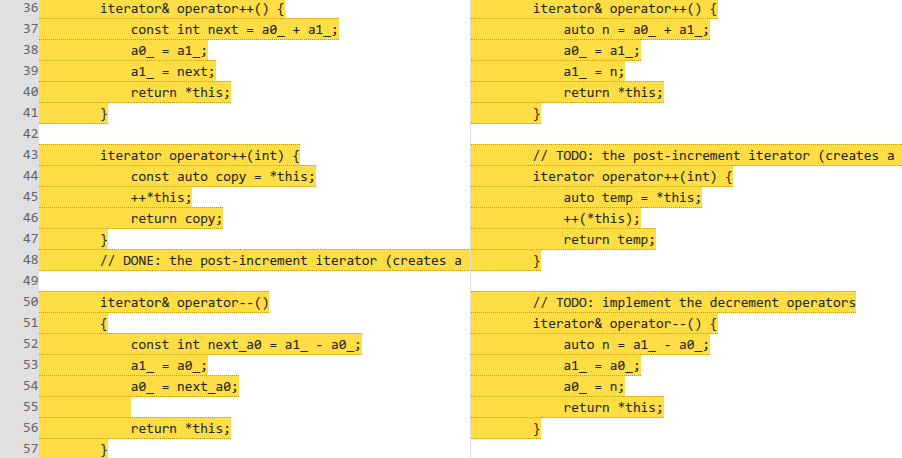
\includegraphics[width=\textwidth]{img/screenshot_variables.png}
  \caption{Two similar code fragments in \texttt{ReCodEx}. \texttt{Comparatrix} gives a lower similarity score due to not recognizing the altered variable names.}
  \label{fig:screenshot_variables}
\end{figure}

\autoref{fig:screenshot_variables} illustrates a short example of two code fragments that are clearly similar, but \texttt{Comparatrix} gives them a lower similarity score.
While both \texttt{Comparatrix} and \texttt{ContrAST} completely ignore comments and whitespace, \texttt{ContrAST} performs a full syntax analysis.
This analysis allows it to, for example, abstract away variable names.
The shown code fragments are nearly identical once the specific identifier names are ignored, allowing our tool to easily match the fragments as a whole.

A common challenge occurs when students are given a template and are supposed to fill in only the missing parts.
The submissions are then identical by default, but the students are not copying from each other.
A similar issue happens when a teacher provides a partial solution during a practical lab session, and students complete the remaining code independently.

This broad spectrum of assignment scenarios makes it impossible to find a single global set of parameters that works perfectly for every task.
We expect that instructors will need to tune the parameters for each problem individually by running the tool on a small set of submissions and inspecting the output.
While this approach will require some initial effort from the teachers, it will prevent a lot of false positives.
Since \texttt{ReCodEx} maintains a centralized catalog of all problems, it would be beneficial to store the parameters within the problem metadata.
This would allow future assignments to reuse the optimized configurations automatically.

\begin{figure}[ht]
  \centering
  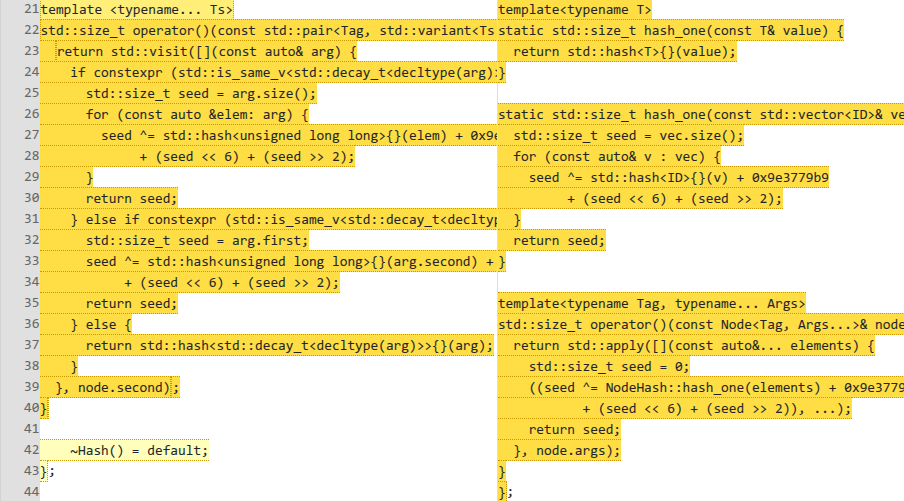
\includegraphics[width=\textwidth]{img/screenshot_hash.png}
  \caption{Two similar code fragments in \texttt{ReCodEx}. The similarity score is moderate, but without broader context, it is impossible to determine whether they represent plagiarism.}
  \label{fig:screenshot_hash}
\end{figure}

Another scenario is presented in \autoref{fig:screenshot_hash}, which displays two moderately similar code fragments.
Because students are solving identical subproblems, the number of logical ways to solve them may be limited.
Alternatively, a specific problem might have a well-known standard solution that many students independently implement.
It is then up to the teacher to look at the context, set the appropriate threshold, and decide if the fragments imply copying.
A reliable strategy for the teacher is to compare the pair against the rest of the submissions to see if the similarity is unique or if many students share the same structure.
The tool is designed to flag potential candidates to cut down the time required for manual inspection, but it cannot replace the teacher's judgment.

\begin{figure}[ht]
  \centering
  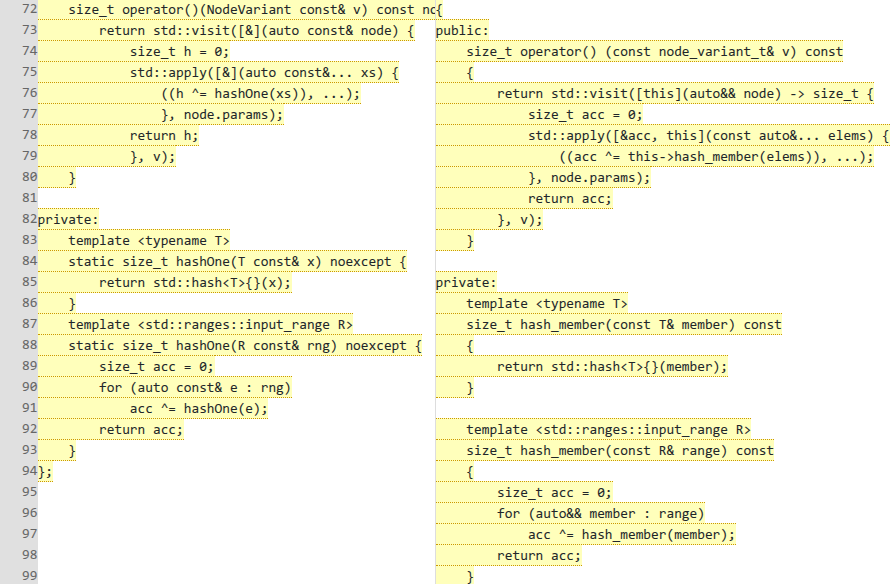
\includegraphics[width=\textwidth]{img/screenshot_syntax.png}
  \caption{Two similar code fragments in \texttt{ReCodEx}. The similarity score is high due to structural syntax analysis rather than literal string matching.}
  \label{fig:screenshot_syntax}
\end{figure}

Finally, \autoref{fig:screenshot_syntax} shows two code fragments matched by \texttt{ContrAST} with a high similarity score, where \texttt{Comparatrix} gives a lower score.
Deep syntax analysis allows the system to ignore minor syntactical changes and focus on the underlying code structure.
By implementing a continuous similarity metric instead of looking for exact literal blocks, the system can successfully flag code fragments that have been modified.

We ran a few test reports with different thresholds on our dataset to verify that the pipeline works end-to-end and that the outputs display correctly inside \texttt{ReCodEx}.
These tests confirmed that setting a high threshold successfully finds obvious copies, while low thresholds generate too many false positives due to shared template code or simple language constructs.
Because our real-world dataset does not have a pre-labeled ground truth, we could not calculate formal precision or recall percentages.
In the upcoming academic year, we plan to hand the tool over to the course instructors so they can use it on live assignments and evaluate the findings directly.

\section{Performance}

The performance tests were executed on an 8-core Intel(R) Xeon(R) Gold 6348 CPU @ 2.60GHz.

We measured the total time required for the entire \texttt{ContrAST} component, which includes loading the data from the saved \texttt{comparatree} instance, running the similarity detection algorithm, and saving the scores back to the database.
We did not include the time spent generating the final report, as it is taking only a few seconds and does not act as a bottleneck in the system.

For CrystalBLEU, we used the conservative abstraction configuration, and for TSED, we used the extreme abstraction configuration, matching the evaluation setup in \autoref{sec:evaluation}.

\begin{figure}
  \centering
  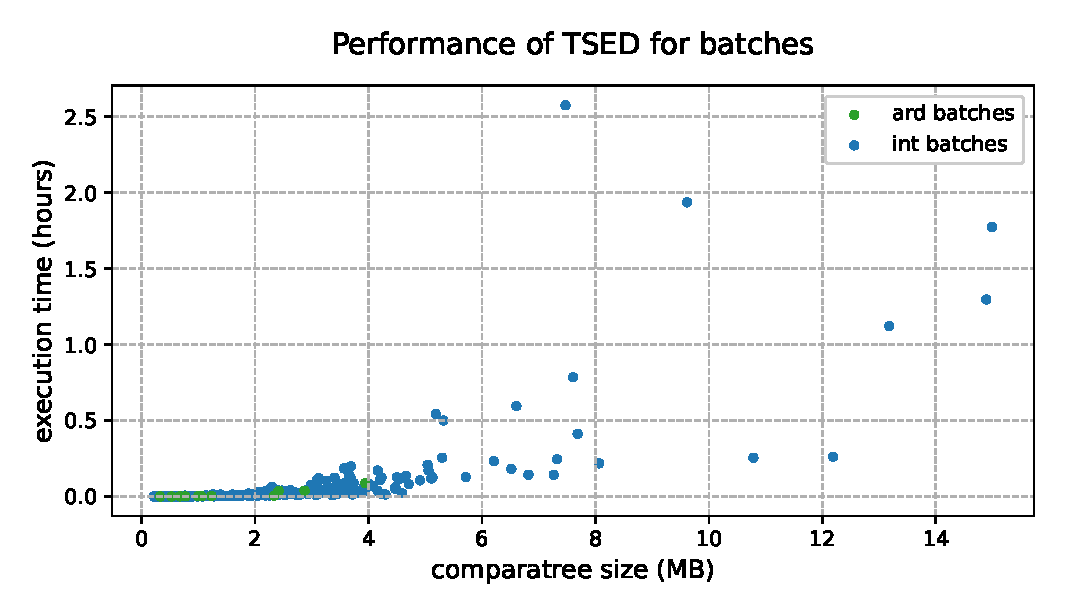
\includegraphics[width=\textwidth]{img/performance-ted-ard-int.eps}
  \caption{Performance of TSED (extreme abstraction) across different assignment batches.}
  \label{fig:performance-ted-batches}
\end{figure}

Based on the benchmarks shown in \autoref{fig:performance-ted-batches} and the nature of the TSED algorithm, the execution time scales poorly with the number of nodes in the \texttt{comparatree} instance.
The runtime is also highly unpredictable, as the performance depends heavily on the specific shape of the trees and how many shared subtrees are assigned to an individual processing thread.

\begin{figure}
  \centering
  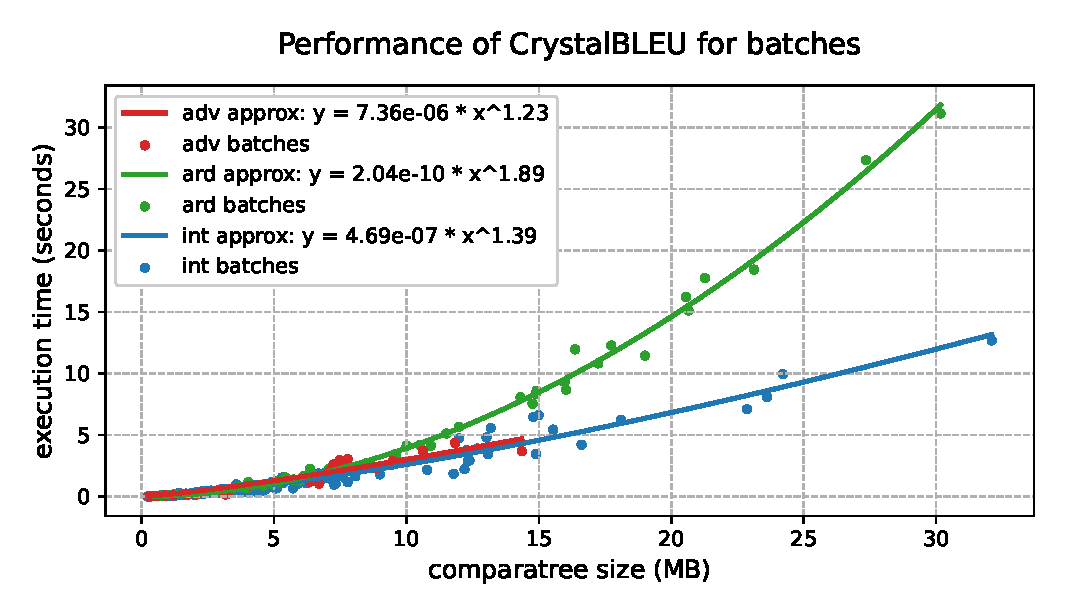
\includegraphics[width=\textwidth]{img/performance-cb-adv-ard-int.eps}
  \caption{Performance of CrystalBLEU (conservative abstraction) across different assignment batches.}
  \label{fig:performance-cb-batches}
\end{figure}

In contrast, CrystalBLEU scales well with the size of the \texttt{comparatree} instance, as shown in \autoref{fig:performance-cb-batches}.
Note that these results do not include any early pre-filtering heuristics, meaning the algorithm is strictly run against all possible pairs of nodes.
Even without filtering, the empirical data suggests a sub-quadratic scaling behavior that performs better than $O(x^2)$ relative to the storage size $x$.

\begin{figure}
  \centering
  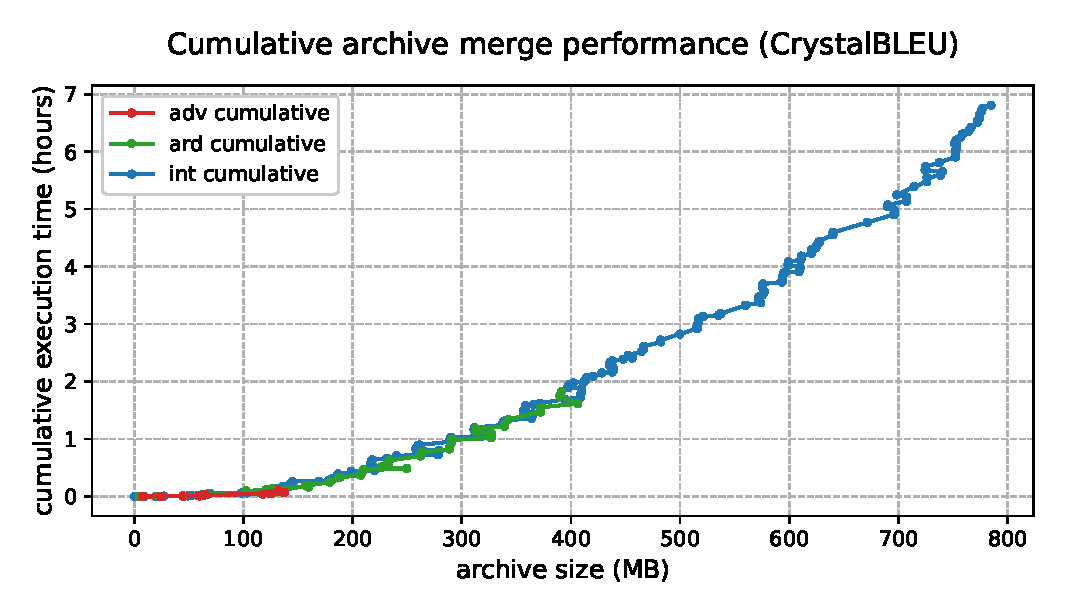
\includegraphics[width=\textwidth]{img/performance-archive-cb-adv-ard-int.eps}
  \caption{Performance of CrystalBLEU (conservative abstraction) on a growing archive of cumulative batches.}
  \label{fig:performance-cb-archive}
\end{figure}

We also measured how CrystalBLEU performs over time on a growing archive of accumulated batches, as displayed in \autoref{fig:performance-cb-archive}.
The data collection ends near the 80~MB mark because we encountered unexpected disk behavior on our testing machine, which caused the test process to terminate.
However, the available data demonstrates that the performance scales efficiently, with each newly appended batch being processed in under 1 minute.
